\documentclass[
    smaller,
    %handout,
]{beamer}

% \usepackage{caption}
% \usepackage{subcaption}
\usepackage{cme193}

\usepackage{fancyvrb}
\fvset{fontsize=\normalsize}
\RecustomVerbatimEnvironment{verbatim}{Verbatim}{}

\usetheme{Boyd}

% \definecolor{sandstone}{rgb}{248,246,234}
% \setbeamercolor{background canvas}{bg=sandstone}


% \AtBeginSection[]
% {
%   \begin{frame}<beamer>
%     %\frametitle{\thesection}
%     \tableofcontents[currentsection]
%   \end{frame}
% }

\newcommand{\lecturenr}{8}
\newcommand{\lecturetitle}{Unit testing, more modules, wrap up}

\newcounter{lectnum}        % Lecture counter
\setcounter{lectnum}{\lecturenr}    % lecture counter

\title{CME 193: Introduction to Scientific Python \\
Lecture \lecturenr: \lecturetitle}
\author{Sven Schmit}
\date{\url{stanford.edu/~schmit/cme193}}
\begin{document}

\maketitle

%% select content here !
%% lecture 1
% 
\section{Administrivia} % (fold)
\label{sec:administrivia}

% \begin{frame}\frametitle{Instructor}
%     \framesubtitle{}

%     Sven Schmit

%     \begin{itemize}
%         \item from the Netherlands
%         \item Third year PhD student in ICME
%         \item Background in Statistics / Mathematics / CS
%         \item Used Python for data science at Stitch Fix
%     \end{itemize}

% \end{frame}

\begin{frame}\frametitle{Quick poll}

    Who has...
    \begin{itemize}
        \item written one line of code?
        \pause
        \item written a \texttt{for} loop?
        \pause
        \item written a \texttt{function}?
        \pause
        \item heard of recursion?
        \pause
        \item heard of object oriented programming?
        \pause
        \item unit testing?
    \end{itemize}
% Know nothing: this might be too difficult
% Know all: might be too easy
\end{frame}

\begin{frame}\frametitle{Feedback}

    If you have comments, like things to be done differently, please let me know
    and let me know asap.

    \vfill

    Questionnaires at the end of the quarter are nice, but they won't help you.

\end{frame}

\begin{frame}\frametitle{Content of course}
\begin{itemize}
    \item Variables
    \item Functions
    \item Data types
    \begin{itemize}
        \item Strings, Lists, Tuples, Dictionaries
    \end{itemize}
    \item File input and output (I/O)
    \item Classes
    \item Exception handling
    \item Recursion
    \item Numpy, Scipy and Matplotlib
    \item Pandas, Statsmodels and IPython
    \item Unit tests
    \item More packages
\end{itemize}

\end{frame}

\begin{frame}\frametitle{Setup of course}

\begin{itemize}
    \item Lectures: first half lecture, second half exercises
    \item Portfolio
    \item Final project
\end{itemize}

\end{frame}

\begin{frame}\frametitle{More abstract setup of course}

    My job is to show you the possibilities and some resources (exercises etc.)

    \vfill

    Your job is to teach yourself Python

    \vfill

    If you think you can learn Python by just listening to me,
    you are grossly overestimating my abilities.

\end{frame}

\begin{frame}\frametitle{Exercises}
    \framesubtitle{}

    Exercises in second half of the class. Try to finish them in class,
    else make sure you understand them all before next class.

    \vfill

    At the end of the course, hand in a portfolio with your solutions for exercises.

    \vfill

    Feel free (or: You are strongly encouraged) to work in pairs on the exercises.
    It's acceptable to hand in the same copy of code for your portfolio if you work in pairs,
    but do mention your partner.

\end{frame}

\begin{frame}\frametitle{Portfolio}
    \framesubtitle{}

    You are required to hand in a portfolio with your solutions to the exercises you attempted.

    \vfill

    This is to show your active participation in class

    \vfill

    You are expected to do at least 2/3rd of the assigned exercises.
    Feel free to skip some problems, for example if you lack some required math background knowledge.

    \vfill

    Don't worry about this now, just save all the code you write.

\end{frame}

\begin{frame}\frametitle{Final project}

    Besides the portfolio, you are required to submit a project,
    due one week after the final class.

    \vfill

    One paragraph proposal due before lecture 4.

    \vfill

    Have fun by working on a project that interests you while learning Python.

    \vfill

    You are encouraged to use material not taught in class:
    we can't cover everything in class.

    \vfill

    No teams :(


\end{frame}

\begin{frame}\frametitle{Final project ideas}

    Some more pointers

    \begin{itemize}
        \item See course website for some possible projects
        \item Focus on Python, not the application (no research)
    \end{itemize}

    Some successful previous projects

    \begin{itemize}
        \item Predicting stock movement, obtaining data using Quandl Api
        \item Crawling and analyzing data from a large forum
        \item Finding recent earthquakes close to a given location using Google maps API and USGS data
    \end{itemize}


\end{frame}

\begin{frame}\frametitle{Workload}

    The only way to learn Python, is by writing Python... \textbf{a lot}.
    So you are expected to put in effort.

    \vfill

    From past experience: If you are new to programming, consider this a hard 3 unit class
    where you will have to figure out quite a bit on your own.
    However, if you have a solid background in another language, this class should be pretty easy.

\end{frame}

\begin{frame}\frametitle{More on workload}

    Expect the first 4 weeks to be very intense: cover all basics.

    After that: reap rewards, focus on project, not as much exercises.

    \vfill

    So: hang on tight, it'll be worth it.

\end{frame}

\begin{frame}\frametitle{To new programmers}

    Be warned, this will be difficult.

    \vfill

    The problem: 8 weeks, 8 lectures, 1 unit. We will simply go too fast.

    \vfill

    Alternative: spend some time learning on your own (Codecademy / Udacity etc).
    There are so many excellent resources online these days.

    Then you can always come back in Fall; this course will be offered again.

\end{frame}

\begin{frame}\frametitle{Misc}

\begin{description}
    \item[Website] \url{stanford.edu/\~schmit/cme193}
    \item[Piazza] Use Piazza for discussing problems. An active user on Piazza has more leeway when it comes to portfolio, as it shows involvement.
    \item[Office hours] After class or by appointment (shoot me an email).
\end{description}

\end{frame}

\begin{frame}\frametitle{References}
    \framesubtitle{}

    The internet is an excellent source, and Google is a perfect starting point.

    \vfill

    The official documentation is also good, always worth a try:
    \url{https://docs.python.org/2/}.

    \vfill

    Course website has a list of useful references.

\end{frame}

\begin{frame}\frametitle{Last words before we get to it}
    \framesubtitle{}

    \begin{itemize}
        \item Work
        \item Make friends
        \item Fail often
        \item Fail gently
    \end{itemize}

\end{frame}

% section administrivia (end)
%% add intro on how to use terminal / cmd prompt
% \section{Introduction} % (fold)
\label{sec:introduction}

\begin{frame}\frametitle{Python}

    \begin{figure}
        \centering
        \centering
        \includegraphics[height=2.5in]{"img/python"}
        \label{fig:xkcd}
    \end{figure}

\end{frame}

\begin{frame}\frametitle{Python}

    \begin{itemize}
        \item Relatively easy to learn
        \item Fast to write code
        \item Intuitive
        \item Very versatile (vs Matlab/R)
        \item Less control, worse performance (vs. C)
        \item Less safety handles, responsibility for user
    \end{itemize}

\end{frame}

% section introduction (end)

% \section{Basics} % (fold)
\label{sec:basics}

\begin{questions}
\titledquestion{The interpreter}
Open the Python interpeter.
What happens when you input the following statements:
    \begin{parts}
        \part \texttt{3 + 1}
        \part \texttt{3 * 3}
        \part \texttt{2 ** 3}
        \part \texttt{"Hello, world!"}
    \end{parts}

\titledquestion{Scripts}
    Now copy the above to a script, and save it as \texttt{script1.py}.
    What happens if you run the script? (try: \texttt{python script1.py}).
    Can you fix this (hint: use the \texttt{print} function)

\titledquestion{More interpreter}
    Explain the output of the following statements if executed subsequently:
    \begin{parts}
        \part \texttt{'py' + 'thon'}
        \part \texttt{'py' * 3 + 'thon'}
        \part \texttt{'py' - 'py'}
        \part \texttt{'3' + 3}
        \part \texttt{3 * '3'}
        \part \texttt{a}
        \part \texttt{a = 3}
        \part \texttt{a}
    \end{parts}

\titledquestion{Booleans}
    Explain the output of the following statements:
    \begin{parts}
        \part \texttt{1 == 1}
        \part \texttt{1 == True}
        \part \texttt{0 == True}
        \part \texttt{0 == False}
        \part \texttt{3 == 1 * 3}
        \part \texttt{(3 == 1) * 3}
        \part \texttt{(3 == 3) * 4 + 3 == 1}
        \part \texttt{3**5 $>=$ 4**4}
    \end{parts}


\titledquestion{Integers}
    Explain the output of the following statements:
    \begin{parts}
        \part \texttt{5 / 3}
        \part \texttt{5 \% 3}
        \part \texttt{5.0 / 3}
        \part \texttt{5 / 3.0}
        \part \texttt{5.2 \% 3}
        \part \texttt{2001 ** 200}
    \end{parts}

\titledquestion{Floats}
    Explain the output of the following statements:
    \begin{parts}
        \part \texttt{2000.3 ** 200} (compare with above)
        \part \texttt{1.0 + 1.0 - 1.0}
        \part \texttt{1.0 + 1.0e20 - 1.0e20}
    \end{parts}

\titledquestion{Variables}
    Write a script where the variable \texttt{name} holds a string with your name.
    Then, assuming for now your name is \emph{John Doe}, have the script output:
    \texttt{Hello, John Doe!} (and obviously, do not use
    \texttt{print "Hello, John Doe!"}.

\titledquestion{Type casting}

    Very often, one wants to ``cast'' variables of a certain type into another type.
    Suppose we have variable \texttt{x = '123'}, but really we would like \texttt{x} to be
    an integer.

    This is easy to do in Python, just use \texttt{desiredtype(x)}, e.g. \texttt{int(x)}
    to obtain an integer.

    Try the following and explain the output
    \begin{parts}
        \part \texttt{float(123)}
        \part \texttt{float('123')}
        \part \texttt{float('123.23')}
        \part \texttt{int(123.23)}
        \part \texttt{int('123.23')}
        \part \texttt{int(float('123.23'))}
        \part \texttt{str(12)}
        \part \texttt{str(12.2)}
        \part \texttt{bool('a')}
        \part \texttt{bool(0)}
        \part \texttt{bool(0.1)}
    \end{parts}

\end{questions}

% \section{Control flow} % (fold)
\label{sec:control_flow}
Disclaimer: Some of the following problems are inspired by problems from \url{www.projecteuler.net}.
Have a look if you are interested, there are some great challenges and Python is an excellent tool for solving them.


\begin{questions}
\titledquestion{Range}
    Type \texttt{range(5)} in the interpreter, what does the interpreter return?
    So what does \texttt{for i in range(5)} mean?

    Let's also find out whether the interpreter can help us understand the object `\texttt{range(5)}' better.
    Type \texttt{type(range(5))} in the interpreter.
    More on this soon!

\titledquestion{For loops}
    Use a \texttt{for} loop to:

    \begin{parts}
        \part Print the numbers 0 to 100
        \part Print the numbers 0 to 100 that are divisible by 7
        \part Print the numbers 1 to 100 that are divisible by 5 but not by 3
        \part Print for each of the numbers $x = 2,\ldots 20$,
            all numbers that divide $x$, excluding $1$ and $x$.
            Hence, for \texttt{18}, it should print \texttt{2 3 6 9}.
    \end{parts}

    Hint: see \url{https://docs.python.org/2.7/library/functions.html#range}.

\titledquestion{Simple while loops} % (fold)
    Instead of using a for loop, use a while loop to:

    \begin{parts}
        \part Print the numbers 0 to 100
        \part Print the numbers 0 to 100 that are divisible by 7
    \end{parts}

\titledquestion{Hangman update 1}
\label{sub:hangman_1}

    Let's reconsider the hangman code we saw in class.\footnote{To obtain the Hangman code, either use \texttt{\$ git clone https://github.com/schmit/hangman.git} (if you have git / use Cloud9)
    or dowload the code directly: \url{https://github.com/schmit/hangman/archive/master.zip}}
    We noted that the computer agent is not very good at guessing.
    Update the code such that the computer guesses `e' first, and 'a' second.

    Use the simulate.py script to see if this improves performance.

    Feel free to play around and see if you can do better!

\titledquestion{While loops} % (fold)
\label{sub:while_loop}

    Use a \texttt{while} loop to find the first 20 numbers that are divisible by 5, 7 and 11, and print them
    Hint: store the number found so far in a variable.

    Pseudo-code:

    \begin{verbatim}
        number found = 0
        x = 11
        while number found is less than 20:
            if x is divisible by 5, 7 and 11:
                print x
                increase number found by 1
            increase x by 1
    \end{verbatim}
% titledquestion while_loop (end)

\titledquestion{More while loops} % (fold)
\label{sub:more_while_loops}

    The smallest number that is divisible by 2, 3 and 4 is 12.
    Find the smallest number that is divisible by all integers between 1 and 10.

% titledquestion more_while_loops (end)

\titledquestion{Collatz sequence} % (fold)
\label{sub:collatz_sequence}

A Collatz sequence is formed as follows:
We start with some number $x_0$, and we find the next number in the sequence by
\[
    x_{i+1} = \begin{cases}
        x_i / 2 & \text{ if $x_i$ is even}\\
        3x_i + 1 & \text{ if $x_i$ is odd}
    \end{cases}
\]
If $x_i = 1$, we stop iterating and have found the full sequence.

For example, if we start with $x_0 = 5$, we obtain the sequence:
\begin{verbatim}
    5 16 8 4 2 1
\end{verbatim}

It is conjectured, though not proven, that every chain eventually ends at $1$.

Print the Collatz sequence starting at $x_0 = 103$.

% titledquestion collatz_sequence (end)
\end{questions}

% section control_flow (end)





%% lecture 2
% \section{Project and Portfolio} % (fold)
\label{sec:project}

% \begin{frame}\frametitle{Some remarks about the final project}
%     \framesubtitle{}

%     \begin{itemize}
%         \item You learn Python by writing Python
%         \item I want to give you freedom to do what you like
%         \item People from very different backgrounds and programming experience
%     \end{itemize}
%     \pause
%     \begin{itemize}
%         \item Do not worry too much about (failing) the project
%         \item Just spend some time outside of class writing Python
%         \item Use your own judgement
%         \item Learn to chain together some concepts
%     \end{itemize}

% \end{frame}

\begin{frame}\frametitle{Proposal}
    \framesubtitle{}

    \begin{itemize}
        \item 1-2 paragraph pdf outlining your project
        \item Upload on coursework dropbox
        \item Due next Wednesday before class
    \end{itemize}

\end{frame}

\begin{frame}\frametitle{Project}

    \begin{itemize}
        \item Content: up to you
        \item Some ideas on course website
        \item Work on your own
        \item Submit source code and brief write-up (updated proposal) on coursework dropbox
        \item Due 10/27 at noon, no late days
        \item See course website
        \item Come ask if things are unclear
    \end{itemize}

\end{frame}

% section project (end)

% \section{Functions} % (fold)
\label{sec:functions}

\begin{frame}\frametitle{Simple example}
    \framesubtitle{}

    \emph{Example:} Suppose we want to find the circumference of a circle with radius
    2.5. We could write

    \codeblock{code/functions_radius0.py}

\end{frame}

\begin{frame}\frametitle{Functions}

    Functions are used to abstract components of a program.

    \vfill

    Much like a mathematical function, they take some input and then do something
    to find the result.

\end{frame}

\begin{frame}\frametitle{Functions: def}
    \framesubtitle{A closer look}

    Start a function definition with the keyword \texttt{def}

    \vfill

    Then comes the function name, with arguments in braces, and then a colon\pause

    \begin{center}
        \texttt{def func(arg1, arg2):}
    \end{center}

\end{frame}

\begin{frame}\frametitle{Functions: body}

    Then comes, indented, the body of the function

    \vfill\pause

    Use \texttt{return} to specify the output

    \begin{center}
        \texttt{return result}
    \end{center}

    \codeblock{code/functions_radius2.py}

\end{frame}

\begin{frame}\frametitle{Return}

    By default, Python returns None

    \vfill

    Once Python hits \texttt{return}, it will return the output and jump out of
    the function

    \pause

    \codeblock{code/functions_return.py}

    What does this function do?

\end{frame}

\begin{frame}\frametitle{How to call a function}
    \framesubtitle{}
    % to update

    Calling a function is simple (i.e. run/execute):

    \texttt{>>> func(2.3, 4)}

\end{frame}

\begin{frame}\frametitle{Quick question}

    What is the difference between \texttt{print} and \texttt{return}?

\end{frame}

\begin{frame}\frametitle{Exercise}
    \framesubtitle{Write your first function}

    \begin{enumerate}
         \item Write a function that prints `Hello, world!'
         \item Write a function that returns `Hello, \texttt{name}!', where \texttt{name}
         is a variable
     \end{enumerate}

\end{frame}

\begin{frame}\frametitle{Exercise solution}
    \framesubtitle{Write your first function}

    \codeblock{code/functions_ex_first.py}

\end{frame}

\begin{frame}\frametitle{Everything is an object}

    Everything is Python is an object, which means we can pass functions:

    \vfill

    \codeblock{code/functions_double.py}

\end{frame}


\begin{frame}\frametitle{Scope}
    \framesubtitle{}

    Variables defined within a function (local), are only accessible within the function.

    \vfill

    \codeblock{code/functions_scope.py}

\end{frame}

\begin{frame}\frametitle{Functions within functions}
    \framesubtitle{}

    It is also possible to define functions within functions, just as we
    can define variables within functions.

    \codeblock{code/functions_within.py}

\end{frame}

\begin{frame}\frametitle{Global keyword}
    \framesubtitle{}

    We could (but should not) change global variables within a function

    \codeblock{code/functions_global.py}

   Question: What is the difference between the last two functions?

\end{frame}

\begin{frame}\frametitle{Scope questions}

    \codeblock{code/functions_scope_q.py}

\end{frame}

\begin{frame}\frametitle{Default arguments}
    \framesubtitle{}

    It is sometimes convenient to have default arguments

    \codeblock{code/functions_default_args.py}

    The default value is used if the user doesn't supply a value.

\end{frame}

\begin{frame}\frametitle{More on default arguments}
    \framesubtitle{}

    Consider the function prototype: \texttt{func(x, a=1, b=2)}

    Suppose we want to use the default value for a, but change b:

    \codeblock{code/functions_default_args2.py}

\end{frame}

\begin{frame}\frametitle{Docstring}
    \framesubtitle{Documentation is important}

    It is important that others, including \emph{you-in-3-months-time} are able
    to understand what your code does.

    This can be easily done using a so called `docstring', as follows:

    \codeblock{code/functions_docstring.py}

    \pause

    We can then read the docstring from the interpreter using:

    \vfill

    \texttt{>>> help(nothing)}

    This function doesn't do anything.

\end{frame}

\begin{frame}\frametitle{Question}
    \codeblock{code/functions_docstring.py}
    \vfill
    Question: what does \texttt{nothing()} return?
\end{frame}

\begin{frame}\frametitle{Lambda functions}
    \framesubtitle{A quick way to define short functions}

    An alternative way to define short functions:

    \codeblock{code/functions_lambda.py}

    \vfill

    Pros:
    \begin{itemize}
        \item One line / in line
        \item No need to name a function
    \end{itemize}

    Try to use these for the homework if you can.

\end{frame}

% section functions (end)



% \section{Functions}
% \begin{frame}
% \frametitle{Functions}
% Functions are used to organize programs into coherent pieces

% \vspace{0.2in}

% In other words, functions are used to generalize or ``abstract" components of a program
% \end{frame}


% \begin{frame}
% \frametitle{Root finding}

% What is a limitation of this code?

% \codeblock{code/while2.py}


% \end{frame}

% \begin{frame}
% \frametitle{Root finding}
% We do not want a $\sqrt{7}$ method, we want a $\sqrt{x}$ method

% \vspace{0.2in}

% We still have the same capabilities (just let $x = 7$), but now our ``abstracted" root finder can be used for more cases
% \end{frame}


% \begin{frame}
% \frametitle{Root finding}

% With this function, we can call \texttt{root(7)}

% \codeblock{code/while3.py}


% \end{frame}

% \begin{frame}
% \frametitle{Root finding}
% More general, we can call \texttt{root(7, 0.1)}:

% \codeblock{code/while4.py}


% \end{frame}


% \begin{frame}
% \frametitle{Root finding}
% Python makes it easy to provide default argument values:

% \codeblock{code/while5.py}


% Can call \texttt{root(3)}, \texttt{root(113, 0.01)}
% \end{frame}

% \begin{frame}
% \frametitle{Root finding}
% A few things to think about:
% \vspace{0.1in}
% \begin{itemize}
% \setlength{\itemsep}{0.1in}
% \item{Are there cases where \texttt{root()} will have an error?}
% \item{Are there cases where \texttt{root()} will run forever? (fail to converge)}
% \item{How else can we generalize the function?}
% \end{itemize}
% \end{frame}


% \begin{frame}
% \frametitle{Basic functions}

% What will happen when this code runs?

% \codeblock{code/func1.py}


% \end{frame}

% \begin{frame}
% \frametitle{Basic functions}

% What about this code?

% \codeblock{code/func2.py}
% \end{frame}


% \begin{frame}
% \frametitle{More function examples}

% \codeblock{code/poly_eval1.py}
% \end{frame}

% \begin{frame}
% \frametitle{More function examples}

% \codeblock{code/poly_eval2.py}
% \end{frame}


% \begin{frame}
% \frametitle{Indentation / white space}

% Python uses indentation (``white space") to group statements

% \vspace{0.15in}

% Each code block is indented the same amount (for loop, while loop, function definition, etc.)

% \vspace{0.15in}

% Python will complain if your indentation is incorrect
% \end{frame}

% \begin{frame}
% \frametitle{Indentation}

% \codeblock{code/indent1.py}

% 2-space or 4-space indentation is standard.

% \end{frame}


% \begin{frame}
% \frametitle{Identation}

% \codeblock{code/indent2.py}

% \end{frame}

% \begin{frame}
% \frametitle{White space}

% Some people like this indentation structure and some people do not.

% \vspace{0.2in}

% ... Python isn't going to stop using it

% \end{frame}


% \begin{frame}
% \frametitle{End}
% \begin{itemize}
% \setlength{\itemsep}{0.05in}
% \item{Assignment 1 is posted on the course web site (due Tuesday 1/14)}
% \item{In-class exercises, python codes from slides, and readings also posted}
% \end{itemize}

% Next time:
% \begin{enumerate}
% \setlength{\itemsep}{0.05in}
% \item{More on Python functions}
% \item{Strings}
% \item{Lists}
% \item{Dictionaries}
% \item{Tuples}
% \end{enumerate}

% \end{frame}

% \section{Lists} % (fold)
\label{sec:lists}

\begin{frame}\frametitle{Lists}

    \begin{itemize}
        \item Group variables together
        \item Specific order
        \item Access items using square brackets: [ ]
    \end{itemize}

    However, do not confuse a list with the
    mathematical notion of a vector.

\end{frame}

\begin{frame}\frametitle{Accessing elements}\framesubtitle{The basics}

    \begin{itemize}
        \item First item: [0]
        \item Last item: [-1]
    \end{itemize}

    \codeblock{code/list_access.py}

    Note: can mix element types!

\end{frame}

\begin{frame}\frametitle{Slicing and adding}\framesubtitle{More on lists}

    \begin{itemize}
        \item Lists can be sliced: [2:5]
        \item Lists can be multiplied
        \item Lists can be added
    \end{itemize}

    % Look into this: confusing!
    \codeblock{code/list_add_slice.py}

\end{frame}

\begin{frame}\frametitle{Multiplication}\framesubtitle{Say what?}

    We can even multiply a list by an integer

    \codeblock{code/list_mult.py}

\end{frame}

\begin{frame}\frametitle{Lists are mutable}

    Lists are mutable, this means that individual elements can be changed.

    \codeblock{code/list_mutable.py}
    % list is unchanged after changing x

\end{frame}

\begin{frame}\frametitle{Copying a list}
    How to copy a list?

    % Look into this, confusing
    \codeblock{code/list_copy.py}.

\end{frame}

\begin{frame}\frametitle{What just happened?}
    Variables in Python really are tags:

    \begin{figure}
        \centering
        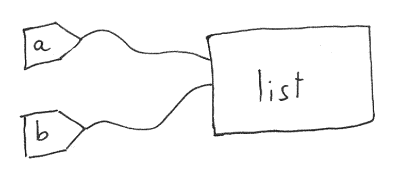
\includegraphics{img/list_tag.png}
    \end{figure}

    So \texttt{b = a} means: \texttt{b} is same tag as \texttt{a}.

    \vfill
    \tiny{Image from \url{http://henry.precheur.org/python/copy_list.html}}

\end{frame}

\begin{frame}\frametitle{Copying a list}

    Instead: we want:
    \begin{figure}
        \centering
        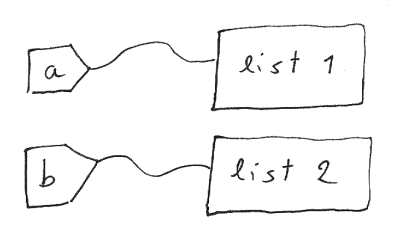
\includegraphics{img/list_tag2.png}
        \caption{\texttt{b = list(a)} or \texttt{b = a[:]}}
    \end{figure}

    \vfill
    \tiny{Image from \url{http://henry.precheur.org/python/copy_list.html}}

\end{frame}

\begin{frame}\frametitle{Copying a list}

    \codeblock{code/list_copy_id.py}

\end{frame}

\begin{frame}\frametitle{Functions modify lists}
    \framesubtitle{}

    Consider the following function:

    \codeblock{code/list_function.py}

    What is printed?

    \vfill \pause

    \texttt{[1, 2, 3]}, \texttt{[0, 2, 3]}

    \emph{Why does the list change, but variables do not?}

\end{frame}

\begin{frame}\frametitle{Why does the list change, but variables do not?}
    We have not changed the tag, only the contents of the list.
    The variable \texttt{l}, that is attached to the list, becomes local.
    The elements however, do not!

    \pause

    What happens in this case?
    \codeblock{code/list_function2.py}
\end{frame}

\begin{frame}\frametitle{More control over lists}

    \begin{itemize}
        \item \texttt{len(xs)}
        \item \texttt{xs.append(x)}
        \item \texttt{xs.count(x)}
        \item \texttt{xs.insert(i, x)}
        \item \texttt{xs.sort()} and \texttt{sorted(xs)}: what's the difference?
        \item \texttt{xs.remove(x)}
        \item \texttt{xs.pop()} or \texttt{xs.pop(i)}
        \item \texttt{x in xs}
    \end{itemize}

    \pause
    All these can be found in the Python documentation, google: `python list'

    Or using \texttt{dir(xs)} / \texttt{dir([])}

\end{frame}

\begin{frame}\frametitle{Looping over elements}

    It is very easy to loop over elements of a list using \texttt{for}, we have
    seen this before using \texttt{range}.

    \codeblock{code/list_loop.py}

\end{frame}

\begin{frame}\frametitle{Looping over elements}
\framesubtitle{and indices}
    Using \texttt{enumerate}, we can loop over both element and index at the same time.

    \codeblock{code/list_loop2.py}

\end{frame}

\begin{frame}\frametitle{Map}
    \framesubtitle{}

    We can apply a function to all elements of a list using \texttt{map}

    \codeblock{code/list_map.py}

\end{frame}

\begin{frame}\frametitle{Filter}
    \framesubtitle{}

    We can also filter elements of a list using \texttt{filter}

    \codeblock{code/list_filter.py}

\end{frame}

\begin{frame}\frametitle{List comprehensions}
    \framesubtitle{The powers of Python}

    A very powerful and concise way to create lists is using \emph{list comprehensions}

    \codeblock{code/list_compr_intr.py}

    This is often more readable than using \texttt{map} or \texttt{filter}

\end{frame}

\begin{frame}\frametitle{List comprehensions}\framesubtitle{Down the rabbit hole}

    \codeblock{code/list_compr.py}

    \pause

    Note how we can have a lists as elements of a list!

\end{frame}

\begin{frame}\frametitle{Implementing map using list comprehensions}

    Let's implement \texttt{map} using list comprehensions
    \pause

    \codeblock{code/list_mymap.py}

    Implement filter by yourself in one of the exercises.

\end{frame}

% section lists (end)


%% lecture 3
% \section{Tuples} % (fold)
\label{sec:tuples}

\begin{frame}\frametitle{Tuples}
    \framesubtitle{}

    Seemingly similar to lists

    \vfill

    \codeblock{code/tuples_basics.py}

\end{frame}

\begin{frame}\frametitle{Tuples are immutable}
    \framesubtitle{}

    Unlike lists, we cannot change elements.

    \codeblock{code/tuples_immutable.py}

\end{frame}

\begin{frame}\frametitle{Packing and unpacking}
    \framesubtitle{}

\codeblock{code/tuples_packing.py}

\end{frame}

\begin{frame}\frametitle{Functions with multiple return values}
    \framesubtitle{}

    \codeblock{code/tuples_functions.py}

\end{frame}


% section tuples (end)

% \section{Dictionaries} % (fold)
\label{sec:dictionaries}

\begin{frame}\frametitle{Dictionaries}
    \framesubtitle{}

    A dictionary is a \emph{collection} of \emph{key-value} pairs.

    \vfill

    An example: the keys are all words in the English language, and their
    corresponding values are the meanings.

    \vfill

    Lists + Dictionaries = \$\$\$

\end{frame}

\begin{frame}\frametitle{Defining a dictionary}
    \framesubtitle{}

    \codeblock{code/dict_def.py}

    Note how we can add more key-value pairs at any time.
    Also, only condition on keys is that they are \emph{immutable}.

\end{frame}

\begin{frame}\frametitle{No duplicate keys}
    \framesubtitle{}

    Old value gets overwritten instead!

    \codeblock{code/dict_duplicate_keys.py}

\end{frame}

\begin{frame}\frametitle{Access}
    \framesubtitle{}

    We can access values by keys, but not the other way around

    \codeblock{code/dict_access.py}

    \pause

    Furthermore, we can check whether a key is in the dictionary by\\
    \texttt{key in dict}

\end{frame}

% \begin{frame}\frametitle{Deleting elements}
%     \framesubtitle{}

%     We can remove a key-value pair by key using \texttt{del}. And we can \texttt{clear}
%     the dictionary.

%     \codeblock{code/dict_del.py}

% \end{frame}

\begin{frame}\frametitle{All keys, values or both}
    \framesubtitle{}

    Use \texttt{d.keys()}, \texttt{d.values()} and \texttt{d.items()}

    \codeblock{code/dict_loops.py}

    So how can you loop over dictionaries?

\end{frame}

\begin{frame}\frametitle{Small exercise}
    \framesubtitle{}

    Print all key-value pairs of a dictionary

    \pause

    \codeblock{code/dict_print.py}

    Instead of \texttt{d.items()}, you can use \texttt{d.iteritems()} as well.
    Better performance for large dictionaries.

\end{frame}

% section dictionaries (end)

% \section{Sets} % (fold)
\label{sec:sets}

\begin{frame}\frametitle{Sets}
    \framesubtitle{}

    Sets are an unordered collection of unique elements

    \codeblock{code/sets_basics.py}

    Implementation: like a dictionary only keys.

    \tiny{from: Python documentation}

\end{frame}

\begin{frame}\frametitle{Set comprehensions}
    \framesubtitle{Similar to lists}

    \codeblock{code/sets_compr.py}

    \tiny{from: Python documentation}

\end{frame}
% section sets (end)

% \section{Strings} % (fold)
\label{sec:strings}

\begin{frame}\frametitle{Strings}
    \framesubtitle{}

    Let's quickly go over \emph{strings}.


    \begin{itemize}
        \item Strings hold a sequence of characters.
        \item Strings are \emph{immutable}
        \item We can slice strings just like lists and tuples
        \item Between quotes or triple quotes
    \end{itemize}

\end{frame}

\begin{frame}\frametitle{Everything can be turned into a string!}
    \framesubtitle{}

    % to edit

    We can turn anything in Python into a string using \texttt{str}.

    \vfill

    This includes dictionaries, lists, tuples, etc.

\end{frame}

\begin{frame}\frametitle{String formatting}
    \framesubtitle{}

    \begin{itemize}
        \item Special characters: \textbackslash n, \textbackslash t,
        \textbackslash b, etc
        \item Add variables: \%s, \%f, \%e, \%g, \%d, or use \texttt{format}
    \end{itemize}

    \codeblock{code/string_format.py}

\end{frame}

\begin{frame}\frametitle{Split}
    \framesubtitle{}

    To split a string, for example, into seperate words, we can use \texttt{split()}

    \codeblock{code/string_split.py}

\end{frame}

\begin{frame}\frametitle{Split}
    \framesubtitle{}

    What if we have a comma seperated file with numbers seperated by commas?

    \codeblock{code/string_split_numbers.py}

    Use the optional argument in \texttt{split()} to use a custom seperator.

    \vfill    \pause

    What to use for a tab seperated file?

\end{frame}

\begin{frame}\frametitle{UPPER and lowercase}
    \framesubtitle{}

    There are a bunch of useful string functions, such as \texttt{.lower()} and \texttt{.upper()} that turn your string in lower- and uppercase.

    Note: To quickly find all functions for a string, we can use \texttt{dir}

    \vfill

    \texttt{text = 'hello'}

    \texttt{dir(text)}

\end{frame}

\begin{frame}\frametitle{join}
    \framesubtitle{}

    Another handy function: \texttt{join}.

    We can use join to create a string from a list.

    \codeblock{code/string_join.py}

\end{frame}

% section strings (end)

% \section{Modules} % (fold)
\label{sec:modules}

\begin{frame}[fragile]\frametitle{Importing a module}
    \framesubtitle{}

    We can import a module by using \texttt{import}

    \vfill

    E.g. \texttt{import math}

    \vfill

    We can then access everything in \texttt{math}, for example the square root
    function, by:

    \vfill

    \texttt{math.sqrt(2)}


\end{frame}

\begin{frame}[fragile]\frametitle{Importing as}
    \framesubtitle{}

    We can rename imported modules

    \vfill

    E.g. \texttt{import math as m}

    \vfill

    Now we can write \texttt{m.sqrt(2)}

\end{frame}

\begin{frame}\frametitle{In case we only need some part of a module}
    \framesubtitle{}

    We can import only what we need using the \texttt{from ... import ...} syntax.

    \vfill

    E.g. \texttt{from math import sqrt}

    \vfill

    Now we can use \texttt{sqrt(2)} directly.

\end{frame}

\begin{frame}\frametitle{Import all from module}
    \framesubtitle{}

    To import all functions, we can use \texttt{*}:

    \vfill

    E.g. \texttt{from math import *}

    \vfill

    Again, we can use \texttt{sqrt(2)} directly.

    \vfill

    Note that this is considered bad practice!
    It makes it hard to understand where functions come from and what if several modules come with functions with same name.

\end{frame}

\begin{frame}\frametitle{Writing your own modules}
    \framesubtitle{}

    It is perfectly fine to write and use your own modules. Simply
    import the name of the file you want to use as module.

    \vfill

    E.g.

    \codeblock{code/modules_first.py}

    \texttt{import firstmodule}\\
    \texttt{firstmodule.helloworld()}

    \vfill

    What do you notice?

\end{frame}

\begin{frame}\frametitle{Only running code when main file}
    \framesubtitle{}

    By default, Python executes all code in a module when we import it.
    However, we can make code run only when the file is the main file:

    \codeblock{code/modules_second.py}

    Try it!

\end{frame}

% section modules (end)


%% lecture 4
% \section{File I/O} % (fold)
\label{sec:file_i_o}

\begin{frame}\frametitle{File I/O}
    \framesubtitle{}

    How to read from and write to disk.

\end{frame}

\begin{frame}\frametitle{The file object}
    \framesubtitle{}

    \begin{itemize}
        \item Interaction with the file system is pretty straightforward in Python.
        \item Done using \emph{file objects}
        \item We can instantiate a file object using \texttt{open} or \texttt{file}
    \end{itemize}

\end{frame}

\begin{frame}\frametitle{Opening a file}
    \framesubtitle{}

    \texttt{f = open(filename, option)}

    \vfill

    \begin{itemize}
        \item filename: path and filename
        \item option:
            \begin{description}
                \item['r'] read file
                \item['w'] write to file
                \item['a'] append to file
            \end{description}
    \end{itemize}

    \vfill

    We need to close a file after we are done:
    \texttt{f.close()}

\end{frame}

\begin{frame}\frametitle{with open() as f}
    \framesubtitle{}

    Very useful way to open, read/write and close file:
    \codeblock{code/fileio_with.py}

\end{frame}

\begin{frame}\frametitle{Reading files}
    \framesubtitle{}

    \begin{description}
        \item[read()] Read entire line (or first $n$ characters, if supplied)
        \item[readline()] Reads a single line per call
        \item[readlines()] Returns a list with lines (splits at newline)
    \end{description}

    \pause

    Another fast option to read a file
    \codeblock{code/fileio_loopread.py}

\end{frame}

\begin{frame}\frametitle{Writing to file}
    \framesubtitle{}

    Use \texttt{write()} to write to a file

    \codeblock{code/fileio_write.py}

\end{frame}

\begin{frame}\frametitle{More writing examples}
    \framesubtitle{}

    \codeblock{code/fileio_writelist.py}

\end{frame}

% section file_i_o (end)

% \section{Classes} % (fold)
\label{sec:classes}

\begin{frame}\frametitle{Defining our own objects}
    \framesubtitle{}

    So far, we have seen many objects in the course that come standard with Python.

    \begin{itemize}
        \item Integers
        \item Strings
        \item Lists
        \item Dictionaries
        \item etc
    \end{itemize}

    \pause

    But often one wants to build (much) more complicated structures.

\end{frame}

\begin{frame}\frametitle{Hangman example}

    Objects:
    \begin{itemize}
        \item Game
        \item Agents (different versions)
    \end{itemize}
\end{frame}

% \begin{frame}\frametitle{Consider `building' a house in Python}
%     \framesubtitle{Analogy}

%     Suppose you have a program that needs to store all information about houses.
%     How are we storing all information about this house?
%     \pause
%     \begin{itemize}
%         \item A house might be a list with two elements, one for rooms, one for construction information
%         \item house = [\{bathroom: ..., kitchen: ...\}, [brick, wood, ...]]
%         \pause
%         \item For the rooms we might again want to know about what's in the room, what it's made off
%         \item So bathroom = [materials, bathtub, sink], where materials is a list
%     \end{itemize}
%     \pause
%     We get a terribly nested structure, impossible to handle!

% \end{frame}

% \begin{frame}\frametitle{Object Oriented Programming}
%     \framesubtitle{}

%     Construct our own objects

%     \begin{itemize}
%         \item House
%         \item Room
%         \item etc
%     \end{itemize}

%     \pause\vfill

%     \begin{itemize}
%         \item Structure in familiar form
%         \item Much easier to understand
%     \end{itemize}

% \end{frame}

\begin{frame}\frametitle{Object Oriented Programming}
    \framesubtitle{}

    Express computation in terms of objects, which are instances of classes
    \begin{description}
        \item[Class] Blueprint (only one)
        \item[Object] Instance (many)
    \end{description}

    \pause\vfill

    Classes specify attributes (data) and methods to interact with the
    attributes.

\end{frame}

\begin{frame}\frametitle{Python's way}
    \framesubtitle{The simple way}

    In languages such as C++ and Java: data protection with
    private and public attributes and methods.

    \vfill

    Not in Python: only basics such as inheritance.

    \vfill

    Don't abuse power: works well in practice and leads
    to simple code.
\end{frame}

\begin{frame}\frametitle{Simplest example}
    \framesubtitle{Finally some code}

    \codeblock{code/classes_leaf.py}

\end{frame}

\begin{frame}[fragile]\frametitle{Initializing an object}
    \framesubtitle{Constructor}

    Define how a class is instantiated by defining the
    \verb|__init__| \textit{method}.

    \vfill

    Seasoned programmer: in Python only one constructor
    method.

\end{frame}

\begin{frame}\frametitle{Initializing an object}
    \framesubtitle{An example}
    The init or \textit{constructor} \textit{method}.

    \codeblock{code/classes_init.py}

    Note how we \textit{access} object \textit{attributes}.

\end{frame}

\begin{frame}\frametitle{Self}
    \framesubtitle{}

    The \texttt{self} parameter seems strange at first sight.
    \vfill
    It refers to the the object (instance) itself.
    \vfill
    Hence \texttt{self.color = color} sets the color of the object
    \texttt{self.color} equal to the variable \texttt{color}.
    \vfill

\end{frame}

\begin{frame}\frametitle{Another example}
    \framesubtitle{}
    Classes have \textit{methods} (similar to functions)

    \codeblock{code/classes_stocks.py}

    \pause

    Recall: \textit{list.append()} or \textit{dict.items()}.
    These are simply class methods!

\end{frame}

\begin{frame}\frametitle{Class attributes}
    \framesubtitle{An example}

    \codeblock{code/classes_class_attribute.py}

    Class attributes are shared among all objects of that class.
\end{frame}

\begin{frame}\frametitle{Class hierarchy through inheritance}

    It can be useful (especially in larger projects) to have a hierarchy of classes.

    Example

    \begin{itemize}
        \item Animal
            \begin{itemize}
                \item Bird
                    \begin{itemize}
                        \item Hawk
                        \item Seagull
                        \item ...
                    \end{itemize}
                \item Pet
                    \begin{itemize}
                        \item Dog
                        \item Cat
                        \item ...
                    \end{itemize}
                \item ...
            \end{itemize}
    \end{itemize}

\end{frame}

\begin{frame}\frametitle{Inheritance}

    Suppose we first define an abstract class

    \codeblock{code/classes_animal.py}

\end{frame}

\begin{frame}\frametitle{Inheritance}
    \framesubtitle{Dog}

    We can define sub classes and inherit from another class.

    \codeblock{code/classes_dog.py}

\end{frame}

% \begin{frame}\frametitle{Why inheritance}


%     An abstract class that implements general functionality can be combined with
%     several subclasses that implement details.

%     \pause\vfill

%     Example: statistical package with a general \textit{Model} class.
%     Subclasses can include \textit{Linear regression}, \textit{Logistic regression}, etc.



% \end{frame}

\begin{frame}[fragile]\frametitle{Base methods}
    \framesubtitle{}

    Some methods to override
    \begin{itemize}
        \item \verb|__init__|: Constructor
        \item \verb|__repr__|: Represent the object (machine)
        \item \verb|__str__|: Represent the object (human)
        \item \verb|__cmp__|: Compare
    \end{itemize}

\end{frame}


% \begin{frame}[fragile]\frametitle{More useful methods}
%     \framesubtitle{}

%     Some more on this later!

%     \begin{itemize}
%         \item \verb|__contains__| for the \texttt{in} keyword
%         \item \verb|__iter__| and \verb|next| for iterators
%     \end{itemize}

% \end{frame}

\begin{frame}\frametitle{Example}
    \framesubtitle{Rational numbers}

    Implementing Rational numbers

    \vfill

    \codeblock{code/classes_rat.py}

\end{frame}

\begin{frame}\frametitle{Setup}
    \framesubtitle{}

    What information should the class hold?

    \pause

    \begin{itemize}
        \item Numerator
        \item Denominator
    \end{itemize}

\end{frame}

\begin{frame}[fragile]\frametitle{Init}
    \framesubtitle{Let's start coding}

    Implement the \verb|__init__| method

    \pause\vfill

    \codeblock{code/classes_rat_init0.py}

\end{frame}

\begin{frame}\frametitle{Issues}
    \framesubtitle{}

    Issues?

    \codeblock{code/classes_rat_init0.py}

    \pause\vfill

    Ignore the division by 0 for now, more on that later.

\end{frame}

\begin{frame}\frametitle{Greatest common divisor}
    \framesubtitle{}

    $\frac{10}{20}$ and $\frac{1}{2}$ are
    the same rational.

    \vfill

    Implement a \texttt{gcd(a, b)} function that computes the greatest common
    divisor of $a$ and $b$.

    \vfill

    \codeblock{code/classes_rat_gcd.py}

    Exercise: Verify Euclidean Algorithm

\end{frame}

\begin{frame}\frametitle{Greatest common divisor}
    \framesubtitle{Solution}


    \codeblock{code/classes_rat_init.py}

    \vfill

    Why is this awesome?

\end{frame}

\begin{frame}\frametitle{Representing your class: Operator overloading}

    Implement \texttt{\_\_repr\_\_} or \texttt{\_\_str\_\_}
    early to \texttt{print}

    \vfill

    Debugging

\end{frame}

\begin{frame}[fragile]\frametitle{Operator overloading: adding two Rationals}
    \framesubtitle{}

    Add Rationals just like Ints and Doubles?\\
    \verb|Rational(10,2) + Rational(4,3)|

    To use \texttt{+}, we implement the \texttt{\_\_add\_\_} method

    \vfill

    \codeblock{code/classes_rat_add.py}
\end{frame}

\begin{frame}[fragile]\frametitle{Operator overloading: Comparing}
    \framesubtitle{}

    \verb|__cmp__| compares objects

    \begin{itemize}
        \item If \texttt{self} is smaller than \texttt{other}, return a negative value
        \item If \texttt{self} and \texttt{other} are equal, return 0
        \item If \texttt{self} is larger than \texttt{other}, return a positive value
    \end{itemize}

\end{frame}

\begin{frame}\frametitle{More on Operator Overloading}

    To learn more:

    \vfill

    Google `Python operator overloading'.

\end{frame}

% section classes (end)



%% lecture 5
% \section{Second part of course} % (fold)
\label{sec:second_part_of_course}

\begin{frame}\frametitle{Congrats, we are halfway!}

    Up to now
    \begin{itemize}
        \item Covered the basics of Python
        \item Worked on a bunch of tough exercises
    \end{itemize}

    From now
    \begin{itemize}
        \item Cover specific topics
        \item Less exercises
        \item Time for project
    \end{itemize}

\end{frame}

\begin{frame}\frametitle{Feedback}

    Thanks for the great feedback, very useful

\end{frame}

\begin{frame}\frametitle{Remaining topics}

    \begin{itemize}
        \item Numpy, Scipy, Matplotlib (today)
        \item IPython notebooks, Pandas, Statsmodels, SKLearn
        \item Exception handling, unit testing, recursion
        \item Brief look at some more modules
        \begin{itemize}
            \item Flask
            \item Regex
            \item ... (suggestions welcome)
        \end{itemize}

    \end{itemize}


\end{frame}


% section second_part_of_course (end)
% \section{Numpy} % (fold)
\label{sec:numpy}

\begin{frame}\frametitle{Numpy}
    \framesubtitle{}

    \begin{itemize}
        \item Fundamental package for scientific computing with Python
        \item N-dimensional array object
        \pause
        \item Linear algebra, Fourier transform, random number capabilities
        \item Building block for other packages (e.g. Scipy)
        \item Open source
    \end{itemize}

\end{frame}

\begin{frame}\frametitle{import numpy as np}
    \framesubtitle{The basics}

    Basics:

    \codeblock{code/numpy_basics.py}

    Slicing as usual.

\end{frame}

\begin{frame}\frametitle{More basics}
    \framesubtitle{}

    \codeblock{code/numpy_basics2.py}

\end{frame}

\begin{frame}\frametitle{More basics}
    \framesubtitle{}

    \codeblock{code/numpy_basics3.py}

\end{frame}

\begin{frame}\frametitle{Arrays are mutable}

    \codeblock{code/numpy_mutable.py}

\end{frame}

\begin{frame}\frametitle{Array attributes}
    \framesubtitle{}

    \codeblock{code/numpy_attr.py}

\end{frame}

\begin{frame}[fragile]\frametitle{Basic operations}
    \framesubtitle{}

    Arithmetic operators: \textbf{elementwise} application

    \codeblock{code/numpy_ops.py}

    Also, we can use \verb|+=| and \verb|*=|.

\end{frame}

\begin{frame}\frametitle{Array broadcasting}
    \framesubtitle{}

    When operating on two arrays, numpy compares shapes.
    Two dimensions are compatible when
    \begin{enumerate}
        \item They are of equal size
        \item One of them is 1
    \end{enumerate}

\end{frame}

\begin{frame}\frametitle{Array broadcasting}
    \framesubtitle{An example}

    \begin{figure}
        \centering
        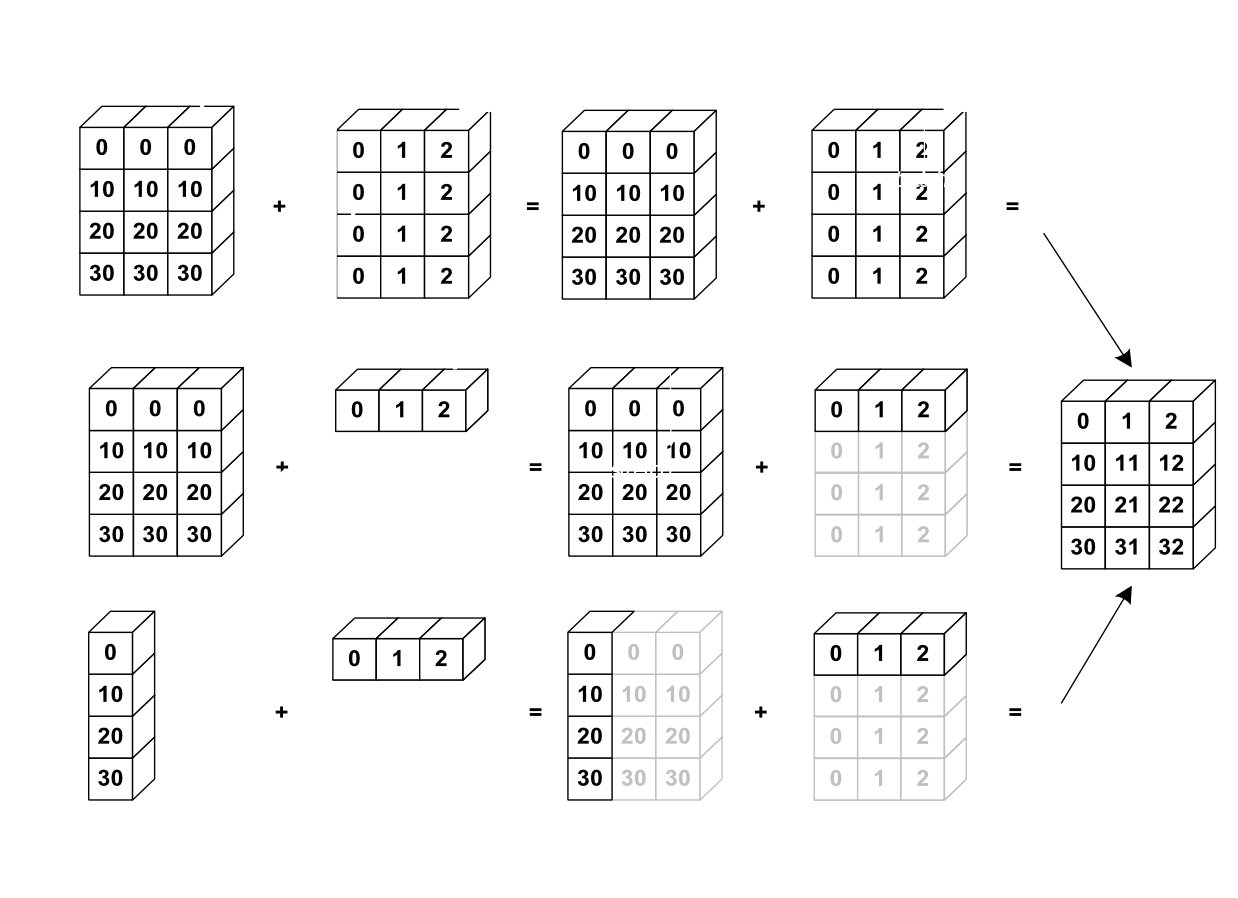
\includegraphics[scale=0.3]{img/broadcasting.png}
    \end{figure}

\end{frame}

\begin{frame}\frametitle{Array broadcasting with scalars}


    This also allows us to add a constant to a matrix or multiply a matrix by a constant


    \codeblock{code/numpy_scalar_ops.py}


\end{frame}

\begin{frame}\frametitle{Vector operations}
    \begin{itemize}
        \item inner product
        \item outer product
        \item dot product (matrix multiplication)
    \end{itemize}

    \codeblock{code/numpy_vector_ops.py}

\end{frame}

\begin{frame}\frametitle{Matrix operations}

    First, define some matrices:

    \codeblock{code/numpy_matrix.py}

\end{frame}

\begin{frame}\frametitle{Matrix operations}

    \codeblock{code/numpy_matrix_ops.py}

\end{frame}



\begin{frame}\frametitle{Operations along axes}
    \framesubtitle{}

    \codeblock{code/numpy_ops2.py}

\end{frame}

\begin{frame}\frametitle{Slicing arrays}
    \framesubtitle{}

    More advanced slicing

    \codeblock{code/numpy_slice.py}

\end{frame}

\begin{frame}\frametitle{Iterating over arrays}
    \framesubtitle{}

    \begin{itemize}
        \item Iterating over multidimensional arrays is done with respect
        to the first axis: \texttt{for row in A}
        \item Looping over all elements:
        \texttt{for element in A.flat}
    \end{itemize}

\end{frame}

\begin{frame}\frametitle{Reshaping}
    \framesubtitle{}

    Reshape using \texttt{reshape}.
    Total size must remain the same.

    \vfill\pause

    Resize using \texttt{resize},
    always works: chopping or appending zeros

    First dimension has `priority', so beware of unexpected results

    \vfill\pause

    Try it!

\end{frame}

\begin{frame}\frametitle{Matrix operations}

\texttt{import numpy.linalg}

\begin{table}
\centering
\begin{tabular}{@{}ll@{}}
    \texttt{eye(3)}& Identity matrix\\
    \texttt{trace(A)}& Trace\\
    \texttt{column\_stack((A,B))}& Stack column wise\\
    \texttt{row\_stack((A,B,A))}& Stack row wise
\end{tabular}
\end{table}

\end{frame}

\begin{frame}[fragile]\frametitle{Linear algebra}
    \framesubtitle{}

\texttt{import numpy.linalg}

\begin{table}
\centering
\begin{tabular}{@{}ll@{}}
    \texttt{qr}& Computes the QR decomposition\\
    \texttt{cholesky}& Computes the Cholesky decomposition\\
    \texttt{inv(A)}& Inverse\\
    \texttt{solve(A,b)}& Solves $Ax = b$ for $A$ full rank\\
    \texttt{lstsq(A,b)}& Solves $\arg\min_x \|Ax-b\|_2$\\
    \texttt{eig(A)}& Eigenvalue decomposition\\
    \texttt{eig(A)}& Eigenvalue decomposition for
    symmetric or hermitian\\
    \texttt{eigvals(A)}& Computes eigenvalues.\\
    \texttt{svd(A, full)}& Singular value decomposition\\
    \texttt{pinv(A)}& Computes pseudo-inverse of A
\end{tabular}
\end{table}
\end{frame}

\begin{frame}\frametitle{Fourier transform}

\texttt{import numpy.fft}

\begin{itemize}
    \item \texttt{fft} 1-dimensional DFT
    \item \texttt{fft2} 2-dimensional DFT
    \item \texttt{fftn} N-dimensional DFT
    \item \texttt{ifft} 1-dimensional inverse DFT (etc.)
    \item \texttt{rfft} Real DFT (1-dim)
    \item \texttt{ifft} Imaginary DFT (1-dim)
\end{itemize}

\end{frame}

\begin{frame}\frametitle{Random sampling}

\texttt{import numpy.random}

\begin{table}
\centering
\begin{tabular}{@{}ll@{}}
    \texttt{rand(d0,d1,...,dn)} & Random values in a given shape\\
    \texttt{randn(d0, d1, ...,dn)} & Random standard normal\\
    \texttt{randint(lo, hi, size)} & Random integers [lo, hi)\\
    \texttt{choice(a, size, repl, p)} & Sample from a\\
    \texttt{shuffle(a)} & Permutation (in-place)\\
    \texttt{permutation(a)} & Permutation (new array)
\end{tabular}
\end{table}

\end{frame}

\begin{frame}\frametitle{Distributions in random}
\texttt{import numpy.random}

    The list of distributions to sample from is quite long, and includes
\begin{itemize}
    \item \texttt{beta}
    \item  \texttt{binomial}
    \item \texttt{chisquare}
    \item \texttt{exponential}
    \item \texttt{dirichlet}
    \item \texttt{gamma}
    \item \texttt{laplace}
    \item \texttt{lognormal}
    \item \texttt{pareto}
    \item \texttt{poisson}
    \item \texttt{power}
\end{itemize}


\end{frame}

% section numpy (end)

% \section{Scipy} % (fold)
\label{sec:scipy}
\begin{questions}
\titledquestion{Least squares} % (fold)
\label{sub:least_squares}

Generate matrix $A \in R^{m \times n}$ with $m > n$.
Also generate some vector $b \in R^m$.

Now find $x = \arg\min_x \|Ax-b\|_2$.

Print the norm of the residual.

% titledquestion least_squares (end)

\titledquestion{Optimization} % (fold)
\label{sub:optimization}

Find the maximum of the function
\[
    f(x) = \sin^2(x-2)e^{-x^2}
\]

% titledquestion optimization (end)


\titledquestion{Pairwise distances} % (fold)
\label{sub:pairwise_dists}

Let $X$ be a matrix with $n$ rows and $m$ columns.
How can you compute the pairwise distances between every two rows?

As an example application, consider $n$ cities, and we are given their coordinates
in two columns.
Now we want a nice table that tells us for each two cities, how far they
are apart.

Again, make sure you make use of Scipy's functionality instead of writing your own routine.

% titledquestion pairwise_dists (end)

\end{questions}

% section scipy (end)

% \section{Matplotlib} % (fold)
\label{sec:section_name}

\begin{frame}
\frametitle{What is Matplotlib?}


\begin{itemize}
    \item Plotting library for Python
    \item Works well with Numpy
    \item Syntax similar to Matlab
\end{itemize}

\end{frame}

\begin{frame}
\frametitle{Scatter Plot}
\lstset{basicstyle=\scriptsize}
\codeblock{code/mpl_line_plot.py}
\begin{figure}[h]
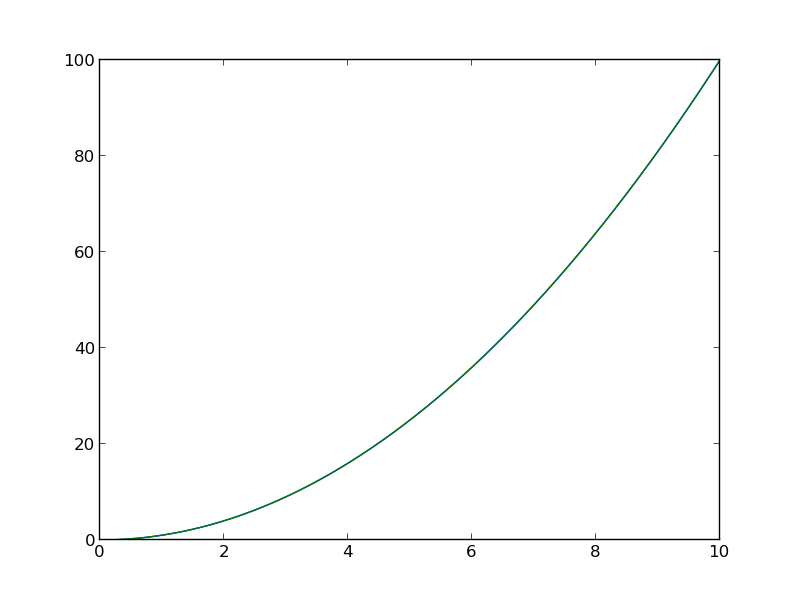
\includegraphics[width=.6\textwidth]{img/line_plot.png}
\end{figure}
\end{frame}

\begin{frame}
\frametitle{Seaborn makes plot pretty}
\lstset{basicstyle=\scriptsize}
\codeblock{code/mpl_line_plot_sns.py}
\begin{figure}[h]
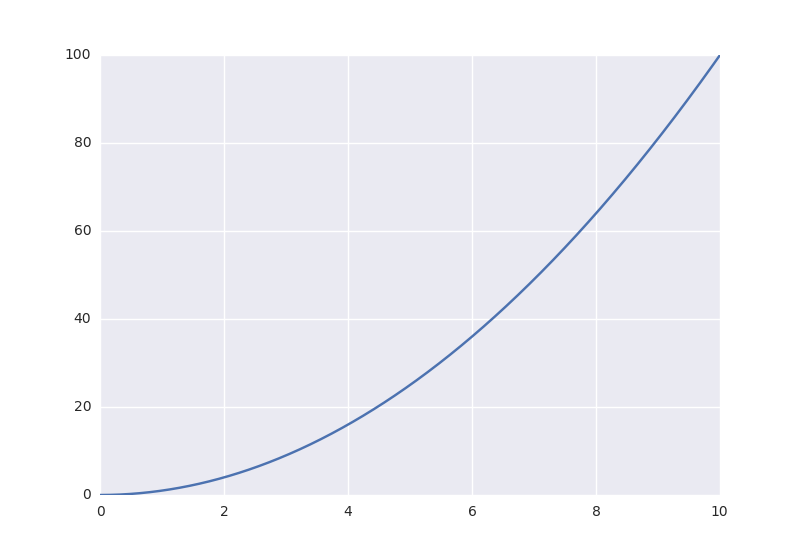
\includegraphics[width=.6\textwidth]{img/lineplot_sns.png}
\end{figure}
\end{frame}


\begin{frame}
Adding titles and labels
\frametitle{Scatter Plot}
\codeblock{code/mpl_line_plot_plus.py}
\end{frame}

\begin{frame}
\frametitle{Scatter Plot}
\begin{figure}[h]
\centering
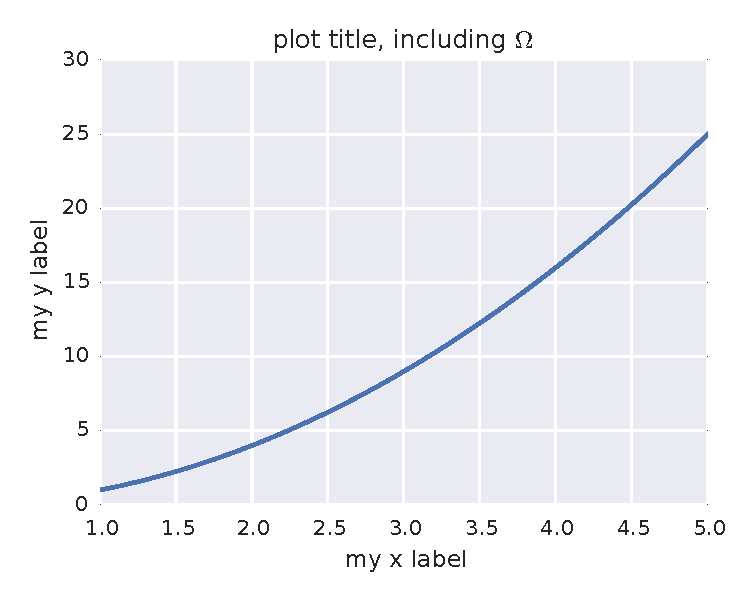
\includegraphics[width=.9\textwidth]{img/line_plot_plus.pdf}
\end{figure}
\end{frame}

\begin{frame}
\frametitle{Scatter Plot}
Adding multiple lines and a legend
\lstset{basicstyle=\small}
\codeblock{code/mpl_line_plot_plus2.py}
\end{frame}

\begin{frame}
\frametitle{Scatter Plot}
\begin{figure}[h]
\centering
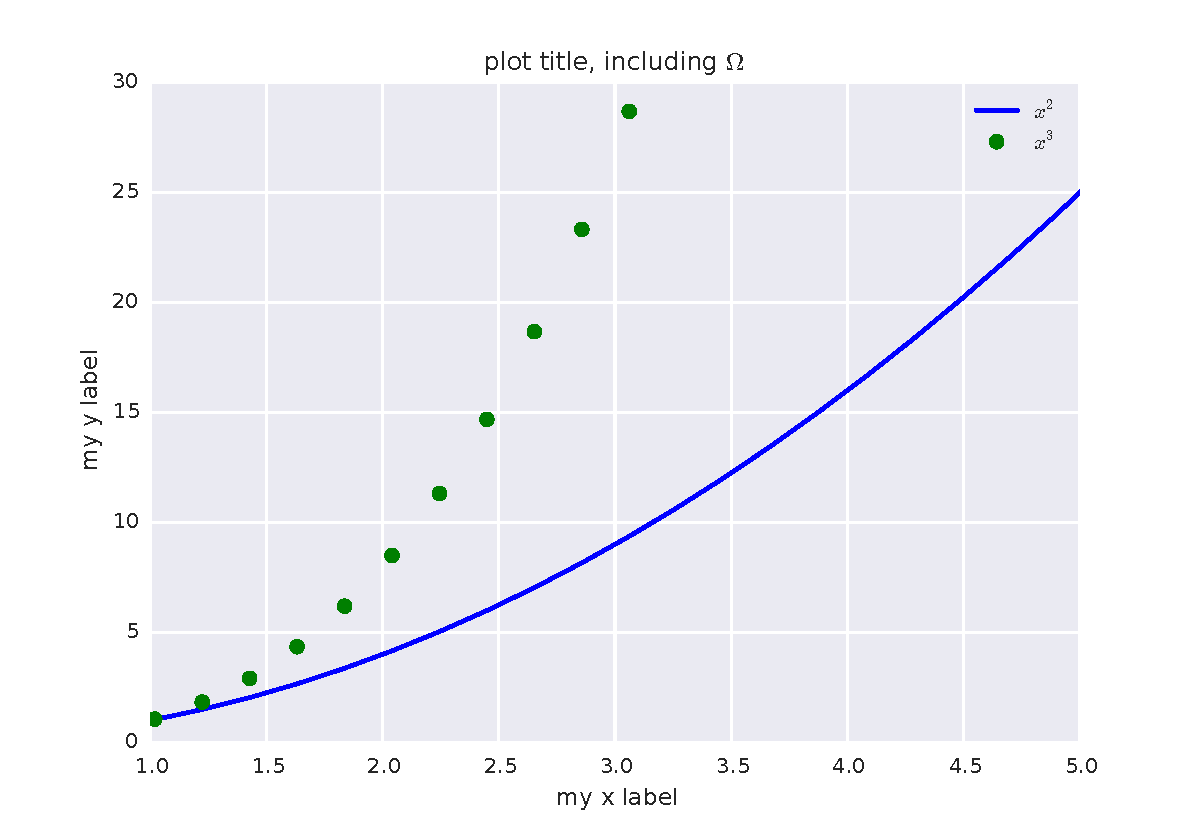
\includegraphics[width=.9\textwidth]{img/line_plot_plus2.pdf}
\end{figure}
\end{frame}


\begin{frame}
\frametitle{Histogram}
\lstset{basicstyle=\small}
\codeblock{code/mpl_histogram.py}
\end{frame}

\begin{frame}
\frametitle{Histogram}
\begin{figure}[h]
\centering
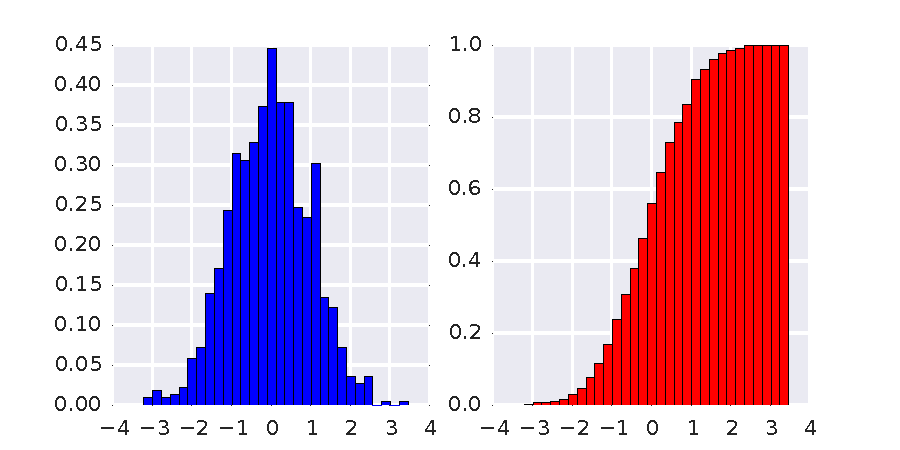
\includegraphics[width=.9\textwidth]{img/histogram.pdf}
\end{figure}
\end{frame}


\begin{frame}
\frametitle{Box Plot}
\codeblock{code/mpl_boxplot.py}
\end{frame}

\begin{frame}
\frametitle{Box Plot}
\begin{figure}[h]
\centering
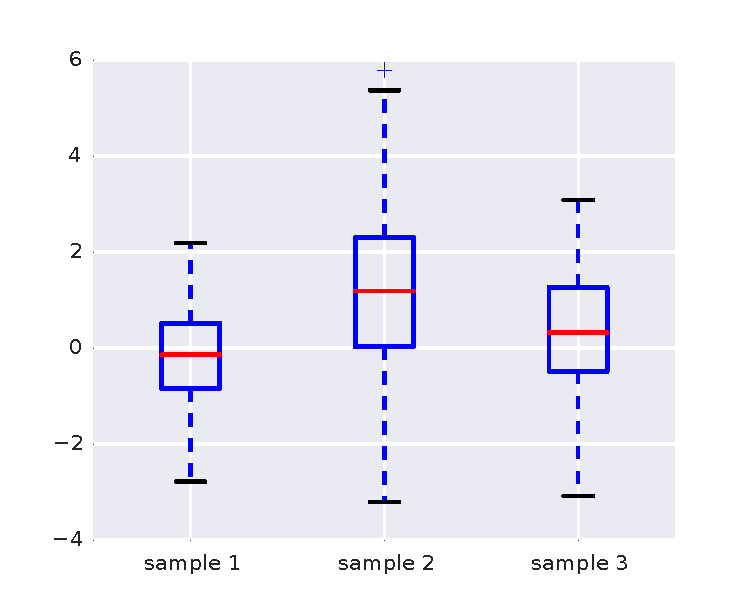
\includegraphics[width=.9\textwidth]{img/boxplot.pdf}
\end{figure}
\end{frame}


\begin{frame}
\frametitle{Image Plot}
\codeblock{code/mpl_imageplot.py}
\end{frame}

\begin{frame}
\frametitle{Image Plot}
\begin{figure}[h]
\centering
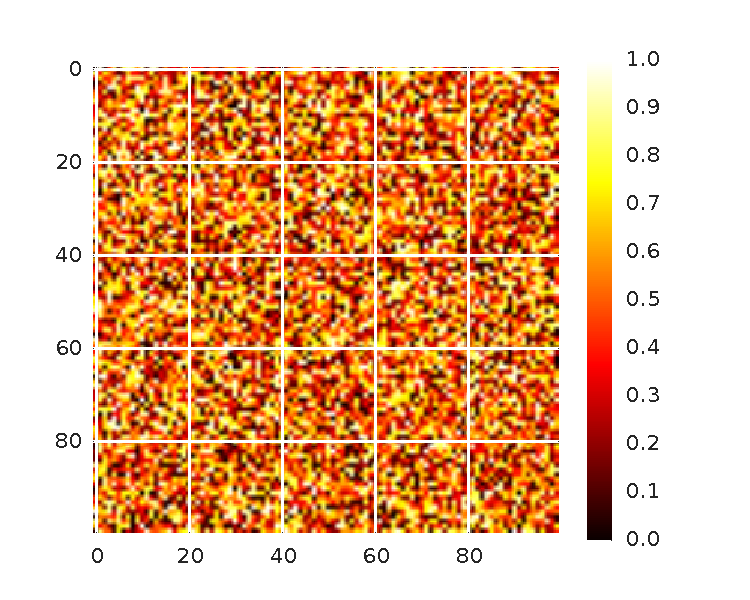
\includegraphics[width=.9\textwidth]{img/imageplot.pdf}
\end{figure}
\end{frame}


\begin{frame}
\frametitle{Wire Plot}
matplotlib toolkits extend funtionality for other kinds of visualization
\codeblock{code/mpl_wire.py}
\end{frame}

\begin{frame}
\frametitle{Wire Plot}
\begin{figure}[h]
\centering
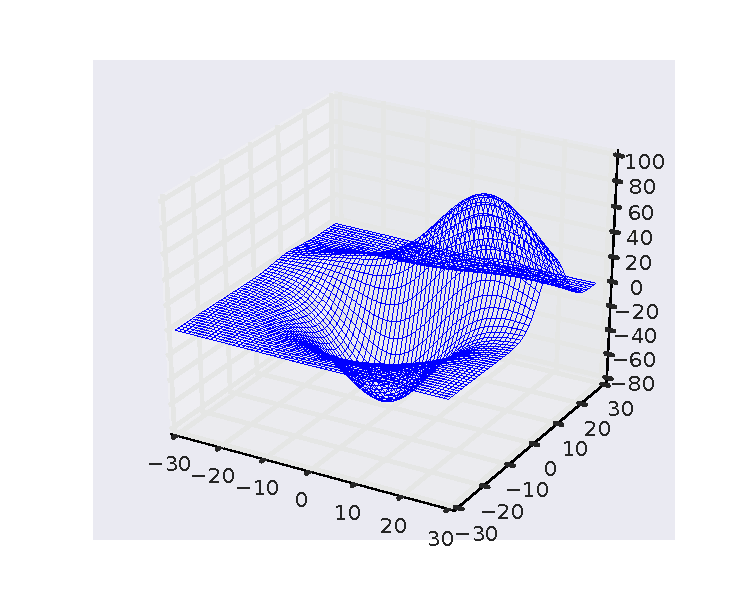
\includegraphics[width=.9\textwidth]{img/wire.pdf}
\end{figure}
\end{frame}

\begin{frame}\frametitle{Possibilities}

A lot is possible, but not always easy to figure out how...

\begin{figure}[h]
\centering
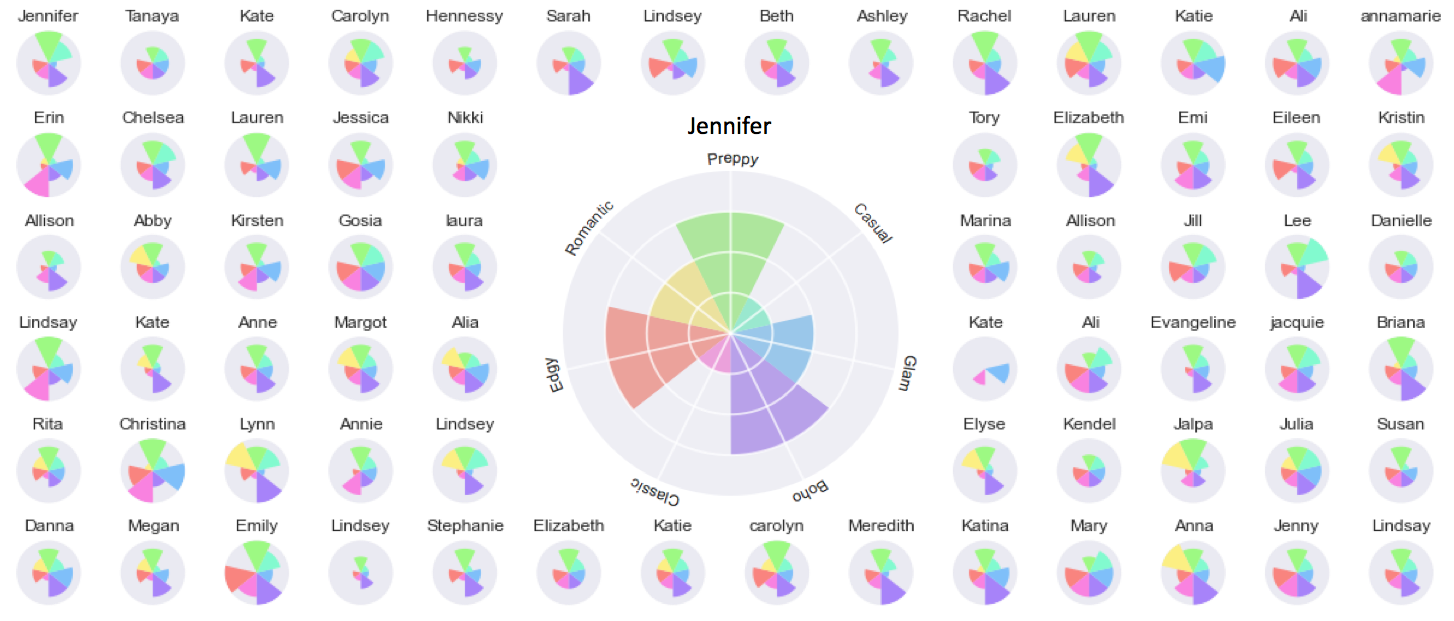
\includegraphics[width=.9\textwidth]{img/sf_vectors.png}
\end{figure}

\end{frame}

% section section_name (end)



%% lecture 6:
% Notebooks
% Pandas
% Statsmodels
% Using iPython Notebook

%% lecture 7:
% \section{Recursion} % (fold)
\label{sec:recursion}

% go slower, add more examples

\begin{frame}\frametitle{Back to control flow}
    \framesubtitle{}

    To execute repetitive code, we have relied on \texttt{for} and \texttt{while}
    loops.
    \vfill
    Furthermore, we used \texttt{if} statements to handle conditional statements.
    \vfill
    These statements are rather straightforward and easy to understand.

\end{frame}

\begin{frame}\frametitle{Recursion}
    \framesubtitle{A new type of functions}

    Recursive function solve problems by reducing them to smaller problems
    of the same form.

    \vfill

    This allows recursive functions to call themselves...

    \pause\vfill

    \begin{itemize}
        \item New paradigm
        \item Powerful tool
        \item Divide-and-conquer
        \item Beautiful solutions
    \end{itemize}

\end{frame}

\begin{frame}\frametitle{First example}
    \framesubtitle{Add numbers}

    Let's consider a trivial problem:

    Suppose we want to add two positive numbers $a$ and $b$, but we can only add/subtract one.

\end{frame}

\begin{frame}\frametitle{First example}
    \framesubtitle{Add numbers}

    Non-recursive solution:
    \codeblock{code/rec_nr_add.py}

\end{frame}

\begin{frame}\frametitle{First example}
    \framesubtitle{Add numbers}

    Recursive solution:

    \begin{itemize}
        \item Simple case: b = 0, return a
        \item Else, we can return 1 + add(a, b-1)
    \end{itemize}
    \pause
    \codeblock{code/rec_add.py}

\end{frame}

\begin{frame}\frametitle{Base case and recursive steps}
    \framesubtitle{Two parts of any recursive function}

    Recursive functions consist of two parts:

    \begin{description}
        \item[base case] The base case is the trivial case that can be dealt with
            easily.
        \item[recursive step] The recursive step brings us slightly closer to
            the base case and calls the function itself again.
    \end{description}

\end{frame}

\begin{frame}\frametitle{Reversing a list}

    How can we recursively reverse a list ([1, 2, 3] $\to$ [3, 2, 1]).

    \begin{itemize}
        \item If list is empty or has one element, the reverse is itself
        \item Otherwise, reverse elements 2 to $n$, and append the first
    \end{itemize}

    \pause

    \codeblock{code/rec_reverse.py}

\end{frame}

\begin{frame}\frametitle{Palindromes}
    \framesubtitle{Another example}

    A palindrome is a word that reads the same from both ways, such as
    \emph{radar} or \emph{level}.
    \vfill
    Let's write a function that checks whether a given word is a palindrome.

\end{frame}

\begin{frame}\frametitle{The recursive idea}
    \framesubtitle{}

    Given a word, such as \emph{level}, we check:
    \begin{itemize}
        \item whether the first and last character are the same
        \item whether the string with first and last character removed are the same
    \end{itemize}

\end{frame}

\begin{frame}\frametitle{Base case}
    \framesubtitle{}

    What's the base case in this case?

    \pause
    \begin{itemize}
        \item The empty string is a palindrome
        \item Any 1 letter string is a palindrome
    \end{itemize}

\end{frame}

\begin{frame}\frametitle{Implementation}
    \framesubtitle{}

    \codeblock{code/rec_palindrome.py}

    \pause

    What is an iterative solution?

\end{frame}

\begin{frame}\frametitle{Numerical integration}
    \framesubtitle{}

    Suppose we want to numerically integrate some function $f$:

    \[
        A = \int_a^b f(x) dx
    \]

    \pause\vfill

    Trapezoid rule:

    \begin{align*}
        A &= \int_a^b f(x) dx\\
         &= \int_a^{r_1} f(x) dx + \int_{r_1}^{r_2} f(x) dx + \ldots + \int_{r_{n-1}}^{b} f(x) dx\\
         &\approx \frac{h}{2}\left((f(a) + f(r_1)) +  h(f(r_1) + f(r_2)) + \ldots + (f(b) + f(r_{n-1}))\right)\\
         &= \frac{h}{2} (f(a) + f(b)) \quad+\quad h (f(r_1) + f(r_2) +\ldots+ f(r_{n-1}))
    \end{align*}
\end{frame}

\begin{frame}\frametitle{Trapezoid rule}
    \framesubtitle{Implementation}

    \codeblock{code/rec_trapezoid.py}

    Forget the math / code:
    This function approximates the area under f between a and b using N points.

\end{frame}

\begin{frame}\frametitle{Key point}

    \begin{itemize}
        \item If function is flat, then we don't need many points.
        \item If function is very wiggly, we need a lot of points.
    \end{itemize}

    So:

    \begin{itemize}
        \item How many points do we need?
        \item What if function is flat in some areas, wiggly in others?
    \end{itemize}

\end{frame}

\begin{frame}\frametitle{Adaptive integration}
    \framesubtitle{Recursive implementation}

    Idea: Adaptively space points based on local curvature of function.

    Areas where function is flat: few points, areas where function is wiggly: many points.

    \pause

    \codeblock{code/rec_adaptint.py}

    Note: we do not need to use trapezoid rule.

\end{frame}

\begin{frame}\frametitle{Pitfalls}
    \framesubtitle{}

    Recursion can be very powerful, but there are some pitfalls:

    \begin{itemize}
        \item Have to ensure you always reach the base case.
        \item Each successive call of the algorithm must be solving a simpler problem
        \item The number of function calls shouldn't explode. (see exercises)
        \item An iterative algorithm is always faster due to overhead of function calls.
         (However, the iterative solution might be much more complex)
    \end{itemize}

\end{frame}

% section recursion (end)



% \section{Exception handling} % (fold)
\label{sec:exception_handling}
\begin{questions}
    \titledquestion{Rational numbers} % (fold)
    \label{sub:rational_numbers}

        Edit your code that implements the \texttt{Rational} class such that
        it raises an exception when the denominator is $0$.

    % titledquestion rational_numbers (end)

    \titledquestion{Wordcount} % (fold)
    \label{sub:wordcount}

        Recall the exercise of finding the 20 most common words in the Complete
        works of Shakespeare.

        Write a script, reusing as much of your code as you can, such that you can specify the filename and k for the k most common words at the command line
        and that the script will print the k most
        common words, and their counts, from the file.

        Make sure you handle errors gracefully, such as a misspecified filename.

    % titledquestion wordcount (end)
\end{questions}
% section exception_handling (end)

% \section{Generators and Iterators} % (fold)
\label{sec:iterators}

\begin{frame}[fragile]\frametitle{For loops}
    \framesubtitle{}

    Recall that in Python we can loop over the elements in a list simply
    by saying

    \begin{verbatim}
        for elem in li:
            # do something
    \end{verbatim}

    We also say that we are iterating over the list.

\end{frame}

\begin{frame}[fragile]\frametitle{Fibonnaci numbers}
    \framesubtitle{}

    Say we want to iterate over the first $n$ Fibonacci numbers:

    \begin{verbatim}
        for elem in fib(n):
            # do something
    \end{verbatim}

    \vfill

    How to implement Fib(n)?

\end{frame}

\begin{frame}[fragile]\frametitle{fib(n)}
    \framesubtitle{}

    We can use our function from the \emph{lists} homework, which returns a list
    with the first $n$ Fibonacci numbers.

    \vfill

    What happens when $n$ is large, say $n = 10^6$ or more generally $n = 10^k$?

    \pause\vfill

    Problem: we have to store the entire list...

    \pause Eventually we will run out of memory.

\end{frame}

\begin{frame}\frametitle{Generators}
    \framesubtitle{The yield keyword}

    Instead, we can use so called generators

    \vfill

    Only difference with functions: use \texttt{yield} instead of \texttt{return}

\end{frame}

\begin{frame}\frametitle{Example: Range}
    \framesubtitle{}

    \codeblock{code/generator_range.py}

\end{frame}

\begin{frame}\frametitle{Advantage over lists}
    \framesubtitle{}

    Note, in this case we never store the entire list.
    \vfill
    This scales much better!
    \vfill
    (though Fibonacci numbers scale poorly, but you get the idea)

\end{frame}

\begin{frame}\frametitle{Back to Fibonacci}
    \framesubtitle{}

    How to write a generator for the Fibonacci sequence?

    \codeblock{code/generator_fib.py}

\end{frame}

\begin{frame}\frametitle{Generators are a simple form of iterators}
    \framesubtitle{}

    Iterators underlie many aspects of Python such as
    \begin{itemize}
        \item List comprehensions
        \item Generators
    \end{itemize}

\end{frame}

\begin{frame}[fragile]\frametitle{Iterators are classes}
    \framesubtitle{}

    \begin{itemize}
        \item Init method to initialize iterator
        \item \verb|__iter__| method to set up the iterator
        \item \verb|next| method to loop over the entries
    \end{itemize}

    More control, but also more code.

\end{frame}

\begin{frame}\frametitle{Range as iterator}
    \framesubtitle{}

    A slight overkill...
    \codeblock{code/iterator_range.py}

\end{frame}

\begin{frame}\frametitle{Fibonacci iterator}
    \framesubtitle{No room for whitespace :(}

    \codeblock{code/iterator_fib.py}

\end{frame}

% section iterators (end)
 % leave out

%% lecture 8: wrap up
\section{Unit testing} % (fold)
\begin{questions}
\label{sec:unit_testing}

    \titledquestion{Factorial} % (fold)
    \label{sub:factorial}
        Write unit tests for the factorial function.

    % titledquestion factorial (end)

    \titledquestion{Prime numbers} % (fold)
    \label{sub:prime_numbers}

        Write a program \texttt{primes.py} that takes two command line arguments,
        $a < b$, and returns all prime numbers between $a$ and $b$ (inclusive).
        Write a seperate test script \texttt{primestest.py} that contains
        unittests for all functions in your script.

    % titledquestion prime_numbers (end)

    \titledquestion{Sorting} % (fold)
    \label{sub:quicksort}
        Write unit tests for a sorting algorithm.
        Test whether your implementation of \texttt{quicksort} passes the tests.

    % titledquestion quicksort (end)
\end{questions}
% section unit_testing (end)

\section{More modules} % (fold)
\label{sec:more_modules}
\begin{questions}
\titledquestion{Regular expressions to find email addresses}

At \url{http://stanford.edu/~schmit/cme193/ex/data/emailchallenge.txt} you find
some text data with some email addresses.
Your task is to write a script that finds these email addresses (and ignores the fake ones).

First, use the \texttt{requests} library to download the data directly into Python (so don't save the file locally).
Then use \texttt{re} to match the email addresses.
Make sure to extract the local part and domain part (before and after \texttt{@}) separately.

You should find 7 email addresses.

Hint: Although written for the Ruby regex, \url{http://rubular.com/} can be very useful
to play around with your pattern. The Python regular expression should be identical or almost identical.

\titledquestion{Flask}

Write a Flask app that displays the current date and time.

Hint: Use the \texttt{datetime} module to get the current time.

\end{questions}
% section more_modules (end)
\section{Wrap up}

\begin{frame}\frametitle{Zen of Python}

    \codeblock{code/wrapup_this.py}

\end{frame}

\begin{frame}\frametitle{Have you fallen in love with Python?}

    `There's nothing wrong with falling in love with a programming language for her looks. I mean, let's face it - Python does have a rockin' body of modules, and a damn good set of utilities and interpreters on various platforms. Her whitespace-sensitive syntax is easy on the eyes, and it's a beautiful sight to wake up to in the morning after a long night of debugging. The way she sways those releases on a consistent cycle - she knows how to treat you right, you know?...'

    \url{https://www.quora.com/Have-I-have-fallen-in-love-with-Python-because-she-is-beautiful}

\end{frame}

\begin{frame}\frametitle{Project and portfolio}

    Please remember: projects and portfolios due next Thursday at noon.

    Coursework checklist:
    \begin{itemize}
        \item Project code (\textbf{py} file(s) or \textbf{zip}).
        \item Project write-up (\textbf{pdf} file (no word!)).
        \item All scripts you wrote for class (\textbf{zip} with all \textbf{py} files). No write up necessary.
    \end{itemize}

\end{frame}

\begin{frame}\frametitle{Feedback}
    \framesubtitle{}

    Thanks a lot!

    Hope you enjoyed the class and learnt a lot!

    \vfill

    Another feedback form:
    \begin{center}
            \url{goo.gl/3onaCL}
    \end{center}
    or via course website

    \vfill

    \texttt{Questions?}

\end{frame}

%% Special slides
% \section{Exercise solutions: control flow} % (fold)
\label{sec:exercise_solutions_control_flow}

\begin{frame}\frametitle{For loops}
    \framesubtitle{Problem}

    Print the numbers 1 to 100 that are divisible by 5 but not by 3

\end{frame}

\begin{frame}\frametitle{For loops}
    \framesubtitle{Solution}

    \codeblock{code/exsol_control_for.py}

\end{frame}

\begin{frame}\frametitle{While loops}
    \framesubtitle{Exercise}

    The smallest number that is divisible by 2, 3 and 4 is 12.
    Find the smallest number that is divisible by all integers between 1 and 10.

\end{frame}

\begin{frame}\frametitle{While loop}
    \framesubtitle{Solution}

    \codeblock{code/exsol_control_while.py}

\end{frame}


\begin{frame}\frametitle{Collatz sequence}
    \framesubtitle{Problem}

    A Collatz sequence is formed as follows:
    We start with some number $x_0$, and we find the next number in the sequence by
    \[
        x_{i+1} = \begin{cases}
            x_i / 2 & \text{ if $x_i$ is even}\\
            3x_i + 1 & \text{ if $x_i$ is odd}
        \end{cases}
    \]
    If $x_i = 1$, we stop iterating and have found the full sequence.

    It is conjectured, though not proven, that every chain eventually ends at $1$.

    Print the Collatz sequence starting at $x_0 = 103$.

\end{frame}

\begin{frame}\frametitle{Collatz sequence}
    \framesubtitle{Solution}

    \codeblock{code/exsol_control_collatz.py}

\end{frame}

% section exercise_solutions_control_flow (end)


\section{Exercises}

\begin{frame}\frametitle{Exercises}
    \framesubtitle{}

    See course website for exercises for this week.

    \vfill

    Let me know if you have any question about exercises or project

    \vfill

    Feel free to email me with questions about project

\end{frame}

\end{document}
